
\section*{Abstract}
\begin{quote}
This chapter presents a hardware design methodology for low-power \gls{cnn} inference, specifically targeting sensor analytics applications. Central to this work is the proposal of the \gls{hf6} quantization scheme and its dedicated hardware accelerator, designed to function as a Conv2D tensor processor. This quantization strategy employs a hybrid number representation, combining standard \gls{fp} and a 6-bit \gls{fp} format. This strategy allows for a highly optimized \gls{fp} \gls{mac}, reducing mantissa multiplication into a multiplexer-adder operation. This research introduces a \gls{qat} method that, in certain cases, offers beneficial regularization effects. The efficacy of this exploration is demonstrated with a regression model, which improves its accuracy despite the applied quantization. For \gls{ml} portability, the custom \gls{fp} representation is encapsulated within a standard format -- a design feature that the proposed hardware automatically processes. To validate interoperability of this approach, the hardware architecture is integrated with TensorFlow Lite, demonstrating compatibility with industry-standard \gls{ml} frameworks and affirming the potential for practical deployment in various sensing applications while maintaining compliance with established \gls{ml} infrastructure.

\end{quote}

\section{Introduction}
\label{sec:introduction}
%%% General intro
There is a growing demand for sensor analytics based on \gls{ml} algorithms. Industry 4.0 and smart city infrastructure leverage \gls{ai} solutions to increase productivity and adaptability~\cite{lom2016industry}. These solutions are powered by advances in \gls{ml}, compute engines, and big data. Therefore, enhancement of these should be considered for research, as they are the machinery of the future.

\glspl{cnn} represent the essential building blocks in 2D pattern analytics. Sensor-based applications such as mechanical fault diagnosis~\cite{li2019sensor,dong2018rolling}, structural health monitoring~\cite{nagayama2007structural}, human activity recognition~\cite{wang2019deep}, hazardous gas detection~\cite{kim2017hazardous} have been powered by \gls{cnn} models in industry and academia. \gls{cnn}-based models, as one of the main types of \gls{ann}, have been widely used in sensor analytics with automatic learning from sensor data~\cite{ince2016real, janssens2016convolutional, abdeljaber2017real, guo2016hierarchical}. In this context, \gls{cnn} models are applied for automatic feature learning, usually, from 1D time series as well as for 2D time-frequency spectrograms. \gls{cnn} models provide advantages such as local dependency, scale invariance, and noise resilience in analytics~\cite{du2014leveraging}. However, \gls{cnn} models are computationally intensive and power-hungry. This is particularly challenging for low-power embedded applications, such as in the \gls{iot} field.

For \gls{ml} inference, dedicated hardware architectures are typically used to enhance compute performance and power efficiency. In terms of computational throughput, \glspl{gpu} offer the highest performance; in terms of power efficiency, \gls{asic} and \gls{fpga} solutions are more energy efficient~\cite{nurvitadhi2017can}. As a result, numerous commercial \gls{asic} and \gls{fpga} accelerators have been proposed, targeting both \gls{hpc} for data-centers and embedded systems applications.

However, most \gls{fpga} accelerators have been implemented to target mid- to high-range \glspl{fpga} for computationally intensive \gls{cnn} models such as AlexNet, VGG-16, and ResNet-18. The main drawbacks of these implementations are power supply demands, physical dimensions, heat sink requirements, air cooling, and high price. In some cases, these implementations are not feasible for ubiquitous low-power/resource-constrained applications.

To reduce hardware there are two types of research~\cite{wu2021low}: the first one is deep compression including weight pruning, weight quantization, and compression storage~\cite{han2015deep,han2015learning}; the second type of research corresponds to a more efficient data representation, also known as custom quantization for dedicated hardware implementation. In this group, hardware implementations with customized 8-bit floating-point computation have been proposed~\cite{mei2017200mhz, wu2021low, lian2019high}. However, these architectures are inadequate for embedded applications, the target devices are high-end \glspl{fpga} and PCIe devices.

Reducing the compute hardware with more aggressive quantization such as binary~\cite{courbariaux2015binaryconnect}, ternary~\cite{lin2015neural}, and mixed precision (2-bit activations and ternary weights)~\cite{colangelo2018exploration} typically incur significant accuracy degradation for very low precisions, especially for complex problems that require precision~\cite{faraone2019addnet}.

In this chapter, it is presented the Hybrid-Float6 quantization and its dedicated hardware design. In this approach, feature maps are represented by a standard \gls{fp} number representation and trainable parameters by 6-bit \gls{fp}. To preserve accuracy, a \gls{qat} method is proposed. For \gls{ml} compatibility/portability, the 6-bit FP can be wrapped into the standard \gls{fp} number representation. It is presented a parameterized tensor processor implementing a pipelined vector dot-product with \gls{hf6}. The proposed hardware extracts the 6-bit representation automatically from the standard \gls{fp} format and performs the computation. The 6-bit \gls{fp} representation uses 4-bit exponent and 1-bit mantissa. This approach enables optimizations in \gls{mac} design by reducing the mantissa multiplication to a multiplexer-adder operation. Moreover, the intrinsic error tolerance of \gls{ann} is leveraged to further reduce the hardware design with approximation. This approach reduces latency, resource utilization, and power dissipation. The embedded hardware/software architecture is integrated with TensorFlow Lite using delegate interface to accelerate \emph{Conv2D} tensor operations. We evaluate the applicability of our approach with a \gls{cnn}-regression model and hardware design exploration for sensor analytics of \gls{shm} for anomaly localization. The embedded hardware/software framework is demonstrated on XC7Z007S, this is the smallest and most inexpensive Zynq \gls{soc} device, see \Fig{fig:workflow}. To the best of my knowledge, this is the first research addressing 6-bit floating-point quantization on \gls{cnn} models and its dedicated hardware design.

\begin{figure}[t!]
	\centering
	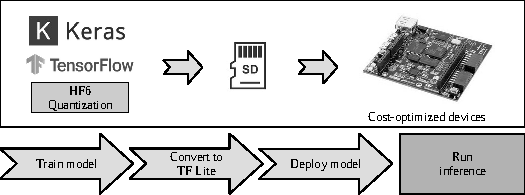
\includegraphics[width=0.5\textwidth]{./chapters/cnn_accelerator/figures/workflow.pdf}
	\caption{The workflow of our approach on embedded FPGAs.}
	\label{fig:workflow}
\end{figure}

The main contributions presented in this chapter are as follows:
\begin{enumerate}
	\item
	
	The Hybrid-Float6 quantization and its dedicated hardware design. It is proposed an optimized hardware \gls{mac} by reducing the mantissa multiplication to a multiplexer-adder operation. The intrinsic error tolerance of \gls{ann} is exploited to further reduce the hardware design with approximation. To preserve model accuracy, it is presented a quantization-aware training method, which provides regularization effects.
	
	\item A custom hardware/software co-design framework for low-power analytics on resource-constrained embedded \gls{fpga}. TensorFlow Lite Micro is integrated in this framework.
	\item A customizable tensor processor as a dedicated hardware for \gls{hf6}. This design computes \emph{Conv2D} tensor operations employing a pipelined vector dot-product with parametrized on-chip memory utilization. For exploration purposes, the compute engine can be synthesized with the proposed \gls{hf6} hardware or with Xilinx LogiCORE IPs (for standard floating-point).
	\item The potential of this approach is demonstrated with a \gls{cnn}-regression model for anomaly localization in \gls{shm} based on \gls{ae}. A hardware design exploration is presented evaluating inference accuracy, compute performance, hardware resource utilization, and energy consumption.
\end{enumerate}

This work is available to the community as an open-source project at:

\url{https://github.com/YaribNevarez/tensorflow-lite-fpga-delegate.git}
